
\input{wsc15style.tex}     % download from author kit.  Style files for wsc formatting. Don't remove this line - required for generating the final paper!

\documentclass{wscpaperproc}
\usepackage{latexsym}
\usepackage{caption}
\usepackage{graphicx}
\usepackage{mathptmx}
\usepackage[utf8]{inputenc}


%****************************************************************************
%% AUTHOR: You may want to use some of these packages. (Optional)
%\usepackage{amsmath}
%\usepackage{amsfonts}
%\usepackage{amssymb}
%\usepackage{amsbsy}
%\usepackage{amsthm}

\usepackage{algorithm,algorithmicx,algpseudocode}
\usepackage{float}
\usepackage{booktabs}



\algnewcommand\And{\textbf{and}}

\usepackage{mathtools}
\DeclarePairedDelimiter\abs{\lvert}{\rvert}%
\DeclarePairedDelimiter\norm{\lVert}{\rVert}%

\newcommand{\specialcell}[2][c]{%
  \begin{tabular}[#1]{@{}c@{}}#2\end{tabular}}


\makeatletter
\let\oldabs\abs
\def\abs{\@ifstar{\oldabs}{\oldabs*}}
\let\oldnorm\norm
\def\norm{\@ifstar{\oldnorm}{\oldnorm*}}
\makeatother

\usepackage{xcolor}
    \usepackage{cite}


\newcommand{\memo}[2]{\textcolor{#1}{#2}}
\newcommand{\added}[2]{\textcolor{#1}{#2}}
%\renewcommand{\memo}[2]{} % uncomment in the final version
%\renewcommand{\added}[2]{#2} % uncomment in the final version
\newcommand{\todo}[1]{\memo{red}{TODO: #1\\}}
\newcommand{\simon}[1]{\memo{green}{Simon: #1\\}}
\newcommand{\jm}[1]{\memo{blue}{JM: #1\\}}
\newcommand{\xrc}[1]{\memo{orange}{XRC: #1\\}}
\newcommand{\new}[1]{\added{orange}{#1}}

\begin{document}

\WSCpagesetup{Montanier, Carrignon, Rubio and Zerr}

\title{Model to study co-evolution of trade an culture}
\maketitle

\begin{figure*}[htb]
{
\centering
Jean-Marc Montanier\\
Simon Carrignon\\ 
Xavier Rubio-Campillo\\
\vspace{12pt}
Barcelona Supercomputing Center\\
Carrer de Jordi Girona, 29, \\
08034 Barcelona, Spain\\
}
\end{figure*}







\section*{ABSTRACT}

\todo{Rewrite later}
In this article our aim is to present a model suitable to test various hypotheses on economic and cultural co-evolution during the Roman Empire. The ultimate goal is to address debates from history of economy such as the type of economical market found in early empires. Agent based modelling is a good way to understand social self-organisation resulting from a large number of interactions. It is used in a wide range of fields of research, from economical market mechanisms to social dynamics. We therefore apply this type of framework to our study.

Here we present a model able it reproduces well known economical and cultural mechanism. Moreover this model can be envisioned to test hypothesis on those mechanisms. Given the appropriate match between the simulations and archaeological and historical data, the results of the model can be validated.


\section{INTRODUCTION}\label{sec:intro}

%XRC trade networks are increasingly being recognised as a key process in ancient Mediterranean
Trades are being increasingly recognised as a key process in the structure of ancient Mediterranean societies. For example, the use of table ware in the Roman empire  has been linked to the trade network~\cite{brughmans_connecting_2010}. Interestingly this trade network has been shown to be a market economy~\cite{temin_market_2001}. The work presented in this paper proposes a framework to further study the relation between trade and culture within the roman empire. This work takes place within the EPNET project~\cite{remesal_epnet_2014}.


%XRC this process played a role in the trajectories of cultural change of the different regions, which were interconnected by trade
The trade possibilities between provinces modify the transmission of culture within each province and between them. The influence can comes from two main sources. First, when a new connection is made between two provinces, new products can arrive in their respective markets. The arrival of new goods naturally changes the rate of adoption of every goods of the market CITE. Moreover, the arrival of new products can lead to their recombination with previous products and therefore the creation of an new item. This further modify the structure of the market of the province. Second, persons are also travelling on the roads of the trade network, each carrying its own culture. Large movements of populations may lead to changes in the cultures. For example, when Roman soldiers were stationing in a province, Roman products such as olive oil were delivered to that province CITE ROMAN DELIVERING OIL. This can lead to the adoption of olive oil in regions that were originally not using it.


%XRC these two elements (cultural transmission and trade networks) are traditionally been studied as isolated systems.
Traditionally cultural transmission and trade are studied distinctively.  On the one hand, the cultural transmission mechanisms studied do not take economical consideration into accounts. The works done are interested in the adoption of various cultural trait without taking into consideration their economical value. On the other hand, trading behaviours are studied within their own framework which are designed to measure the amount of goods exchanged and the value at which they are exchanged. Within these frameworks the cultural transmission between persons is not present.


%XRC this is wrong because blablabla
As it has been stated before, trades influence cultural transmission by modifying both the goods present in a region and the people consuming these goods. On the one side, analysing separately trade and cultural transmission allows to formalize their inner mechanisms and understand their respective dynamics. On the other hand, in order to analyse the adoption of goods within a province one must take into account both trading strategy and cultural transmission. For example, the modification of good's consumption after the rupture of a connection in the trade system is better explained by knowing the local adoption of this good (cultural transmission) and the prices of this good (trade).

%XRC we propose a model of coevolution to explore the deep links between trade and cultural transmission in the ancient Mediterranean
We propose in this article a framework to study the interaction between cultural transmission and trade. This framework should be able first to reproduce well known dynamics of both cultural transmission and trading. Second, to be useful, this framework should be able to compare results obtained by taking cultural or trade into consideration. In order to build this framework we view trade events as part of the culture. The price of a good are then viewed as a cultural trait. This traits can be transmitted and modified along different rules. By this mean, traditional works previously expressed in a trading framework, can be expressed in a cultural evolution framework. Therefore, the dynamics observed on various cultural transmission mechanisms can be straightforwardly compared to dynamics obtained by trading mechanisms. In order to demonstrate the feasibility of this approach we propose a minimal implementation able to reproduce both cultural transmission dynamics and trade dynamics. Additionally we will analyse the results obtained with tools from both economy and cultural evolution.




%Organisation of the paper
\todo{write once we are more sure of what we put}
The paper is organised as follow

\section{PREVIOUS MODELLINGS OF TRADE AND CULTURE}

This section will provide a brief review of the previous approaches to model trade and culture. While non-exhaustive, this review presents the mains trends of the previous work done.

\subsection{Neutral models of cultural change}

The first aspect of our model is focused on the dynamics of cultural change. They comprise the collection of processes that promotes or inhibits the spread of information by social interaction within a population \cite[3]{boyd_origin_2005}. An increasing number of social scientists are using an evolutionary framework to model these dynamics, thus fostering the development of transdisciplinary efforts designed to understand cultural evolution \cite{henrich_evolution_2003}. Archaeology has a rich tradition of evolutionary studies \cite{lycett_cultural_2015}, exploring concepts such as gene-culture coevolution \cite{burger_absence_2007}, diffusion processes \cite{fort_synthesis_2012}, phylogenetic analysis of material culture \cite{obrien_cladistics_2001} or detection of rates of change in the archaeological record \cite{premo_cultural_2014}.

A large percentage of these studies focus on the biases that affect the transmission of cultural traits, including the relevance of intrinsic traits and frequency dependence (e.g. conformism and anti-conformism). 
\jm{to keep it simple, can we say ``evolutionary theory" instead of ``genetic theory" ?}
These analysis are often based on the genetic theory of neutral evolution \cite{neiman_stylistic_1995} and they take neutrality as a null-hypotheses, i.e. variations of traits are strictly explained by their frequency distribution in the population. There exist a large number of works using this model as the starting point to analyse patterns of cultural change in past societies \cite{lipo_neutralitystyle_2001,shennan_ceramic_2001,steele_ceramic_2010,kandler_nonequilibrium_2013,porcic_exploring_2014,crema_approximate_2014}.

Unbiased transmission generates a clear pattern of power law distributions that can be replicated with a simple random copying transmission mechanism \cite{bentley_random_2004}. Within this framework, an individual will copy the traits of a randomly chosen individual with a given probability. This copy can potentially introduce some errors in the acquired trait, which account for innovation processes. The individual will in turn continue to spread these cultural traits which will be further adopted by other individuals. This basic model can be enriched by several additional processes both in the innovation \cite{schillinger_copying_2014,sole_evolutionary_2013,ziman_technological_2003} and the transmission \cite{heyes_social_1994,henrich_evolution_2003}.

In particular, the trade of cultural products within a market system can potentially introduce a dynamics content-related bias linked to the price of the different products. This would also affect the frequency of the product within the population, which in turn would modify its price following a co-evolutionary dynamic.


\subsection{Models of Trade}

%Hopkins 1980: structure of tax system. two hypothesis. 1)taxation increased volume of trade in the empire? 2) tax-exporting province (recently integrated province) had to export to pay tax. roman supported by many small taxes. Not sure to cite it

Previous historical and archaeological studies to model trade in the ancient Mediterranean societies have focus on descriptive approaches ~\cite{hopkins_taxes_1980,temin_market_2001,terpstra_trade_2011,temin_economy_2006,wilson_approaches_2009,scheidel_model_2007,kessler_organization_2007}. 
These works have conclude that the Roman economy was a type of market economy where a variety of small tightly connected markets had loose connections between them~\cite{temin_market_2001,temin_economy_2006,wilson_approaches_2009}. 
Based on these conclusions, further works have attempt to define more exactly which type market economy was in use, i.e. was it close to our market economy or remote ? 

Among the various works done with this objective, few are studying the interactions between economy and cultural change in the Roman empire~\cite{terpstra_trade_2011,kessler_organization_2007,scheidel_model_2007}. 
An analysis based on historical documents has revealed the importance of economical and social institutions for the efficiency of trades of grains in the early Roman Empire~\cite{kessler_organization_2007}. The same type of analysis has also revealed the importance of a number of key factors (such as commercial development, population growth and geographical mobility) for the growth of income and population in the Roman Italy~\cite{scheidel_model_2007}. Finally, a micro-economic model has determined the importance of reputation and threat of expulsion from a trade network as mechanisms to maintain the overall efficiency of the trade network~\cite{terpstra_trade_2011}. These works therefore reveal the strong relation between trade and cultural change in the Roman empire.


However, a limitation of the previous works is the impossibility to test the conclusions reached by the authors. The models proposed reflects only the view of the authors on the data analysed. A new type of model would be necessary to go beyond the interpretation, and allow the verification of the conclusions reached. These models should be able to generate data which is then qualitatively compared to the real historical data. By this mean, if a factor is really important in the economical network, its removal from the model will lead to data qualitatively different from the historical data. The Agent Based Models (ABM) methodology offers a way to produce this kind of model~\cite{lake_trends_2014}.

Based on this tool a relatively complex and exact modelisation of the prehispanic Pueblo societies has been proposed~\cite{kohler_modelling_2012}. This work offers an ABM integrating numerous effects such as food consumption, production and landscape. The questions studied are  numerous and some works are performed on the economical system and its ties with social transmissions~\cite{kobti_emergence_2006,cockburn_simulating_2013}. However the work done in this project consider a pre-market society in a specific village which makes it difficult to reach more general conclusions, notably applicable to the Roman Empire.

%kobti 2012 la meme que kobti 2006 ?
%	pour 2006: etude de l'apparition d'inegalite

\subsection{Models of Trade and Culture}

\jm{tried a justification of co-evolutionary framework but I find it too light. ideas ?}

Ultimately, we aim to create a model to study the relation between cultural change and trade networks within the Roman Empire. Examples of questions that could be asked to our model are: What is the relation between distances in the trade network and cultural changes ? Did anti-conformism promote the adaptation of new products coming from remote provinces ? In order to answer these questions the model used has to take into account both cultural effects and trade influence. More precisely, the variations in these two aspects should be modelled and should influence each other.  Therefore, in order to answer the questions targeted we need a co-evolutionary model able to take into account both trade and cultural changes. 

To the best of our knowledge two works have previously proposed frameworks that could be used to model the co-evolution of trade and culture~\cite{bentley_specialisation_2005,macmillan_agent-based_2008}. The first proposes a relatively simple model which is limited by 2 products, a fixed behaviour of the agents and a limited variation of cultural mechanisms. The second proposes a more complete model including a large number of goods (certain being essential and the others non-essential), but suffer from a greater complexity and the absence of the notion of trade networks. Moreover, these works do not compare the dynamics obtained to the previous studies on cultural change and trading mechanisms.

The model presented in this work aims to offer a framework for the co-evolution of culture and trades which relies on a low number of parameters. It is not within the scope of this article to answer the questions asked at the beginning of this section as they require specific implementations of the model proposed. However, the article will focus on the presentation of the framework, its justification and more importantly its validation by reproducing previous results obtained on cultural change and trade mechanisms.



\section{MODEL DESCRIPTION}

The model proposed is a Multi-Agent Based model including agents and products. It revolves around the value that agents associate to products through cultural change mechanisms, trade mechanisms or both. Depending on the question studied, the value can reflect the interest of the agent for the good or it can be the price at which the agent evaluate this good. The agents are also endowed with limited storage abilities for each good that can be produced. 

More formally the model is composed of a population $Pop$ of $m$ agents, each defined by 2 vectors of size $n$. The first corresponds to the quantity of each good that the agent $i$ possesses: 
$$\forall i \in Pop, \quad Q^i = (q^i_1,\cdots,q^i_n) $$

where $Q^i$ is the total list of possessions of agent $i$, and $q^i_j$ is the number of goods of type $j$ that agent $i$ posses.

The second vector reflects the estimation of the value of a product that an agent $i$ makes.
$$\forall i \in Pop, \quad V^i = (v^i_1,\cdots,v^i_n) $$
where $V^i$ is the total list of estimated values of agent $i$, and $v^i_j$ is the value that agent $i$ associates to the goods of type $j$.

On top of these elements three processes are included : \textit{production}, \textit{imitation} and \textit{innovation}. The \textit{production} process describe the creation of goods by the agent. Once a good is produced by an agent $i$ it is added its quantity vector ($Q^i$). Within the \textit{imitation} process an agent $i$ can copy the value vector ($V^j$) of an agent $j$, where $j \neq i$. Finally, the \textit{innovation} process also modifies the value vector $V^i$ of an agent, but it differs from the \emph{imitation} process in that the modification is done without reference to the other agents. 

This scheme allow us to have a model achieving the two main goals listed in section~\ref{sec:intro}. The first goal is to be able to implement and compare various cultural transmission mechanisms as well as trade mechanisms within the same framework. We argue that this is possible in our framework by modifying only the three key processes i.e. production, imitation and innovation. Moreover, thanks to the use of a unique $V^i$ vector, it is possible to compare the outcomes of different combinations of production, imitation and innovation mechanisms. The second goal is to produce a model composed of a low number of parameter. Our model is composed of only three processes and two vectors which is significantly less complex than previous models.


\section{EXPERIMENTAL SETUP}


In order to validate our model we first reproduce common results from the literature on cultural transmission. We then show that it is possible to transform our model to fit processes that are economically sound. In the following, we present the two set of implementations of the three core processes (production, imitation and innovation) that were used in our experiments.

\subsection{Cultural Transmission}

The first set of implementations of the core processes aims at reproducing a common result from the literature on cultural change.
In this article, the cultural change hypothesis tested is the neutral hypothesis, which has been shown to be followed by multiple cultural phenomenons~\cite{bentley_random_2004,bentley_specialisation_2005,mesoudi_random_2009}. Under this hypothesis, the production of goods is not tested, as a consequence, in this set of implementation, the \emph{production} process does not modify the content of the quantity vector of the agents.
The \emph{imitation} process used is  ``random copy'', which has been implemented as follow: each agent has a low probability to pick randomly one agent among all and copy its vector of values. The \emph{innovation} process, termed ``unbounded'', is triggered with a low probability and draw a new random value to replace an element $v^i_j$. The imitation and innovation probabilities are presented with other parameters in table~\ref{tab:parameters}.

The neutral hypothesis states that the ``random copy'' and the ``unbounded'' innovation process used under a fixed population size, leads to a repartition of cultural variants termed ``power law''. This distribution is characterized by a small number of very frequent traits and a large number of very rare traits. Since this hypothesis has been verified in previous works implementing similar \emph{imitation} and \emph{innovation} mechanisms, we expect in this work the observation of a similar ``power law' distribution. More formally, this distribution is formalised as : $$P(v)=C/v^\alpha $$, where $v$ is the number of time a variant has been repeated, $P(v)$ the probability to find that variant, $C$ a constant, $\alpha$ a variable. 

\subsection{Trading Model}\label{sec:trade}

The second set of implementations of the core processes aims at producing economical dynamics. We are interested in the exchange of products between agents when they can modify the prices at which they sell and buy products. We want to implement simple processes leading to the convergence of prices to values acceptable by all agents.

\paragraph{Production}
In this set of implementations, each agent is producing only one type of good. The type good produced by an agent is assigned to it at the beginning of the simulation and does not change. 

\paragraph{Imitation}
Within this set of implementations, the key ideas behind the imitation mechanism is to copy the agents which are the best at trading. To do so, the imitation mechanism used takes into account the value vector of the other agents and relies on two new notions: \emph{need} and \emph{score}. 

The \emph{need} is a quantity of product that each agent tries to obtain. This quantity is different for each product but the need for a product is the same for all agents:
$$ N = (n_1, \cdots, n_r) $$ 

The \emph{score} $s^i$ of an agent $i$ reflects the ability of this agent to obtain the products it needs. It is maximum when the quantity vector of an agent is equal to its need vector and lower proportionally to the distance between the need vector and the quantity vector.  It is formally computed as follow for agent $i$:

\begin{equation}\label{eq:score}
s^i = \begin{cases}
 s_{max}=1 & \text{if $q^i_j = n_j$}\\
1 -\dfrac{\abs{q^i_j - n_j}}{ \sqrt{\abs{(q^i_j)^2-(n_j)^2}}} & \text{if $q^i_j \neq n_j$}
\end{cases}
\end{equation}


This function ensures that each good count for the same proportion in the final score (i.e.: managing to get only the right amount of a good with a high ``need'' value will not give a better score to the agent). The values of $s^i$ obtained for different need values are depicted in figure~\ref{fig:fit}.


\begin{figure}[htp]
	\begin{center}
		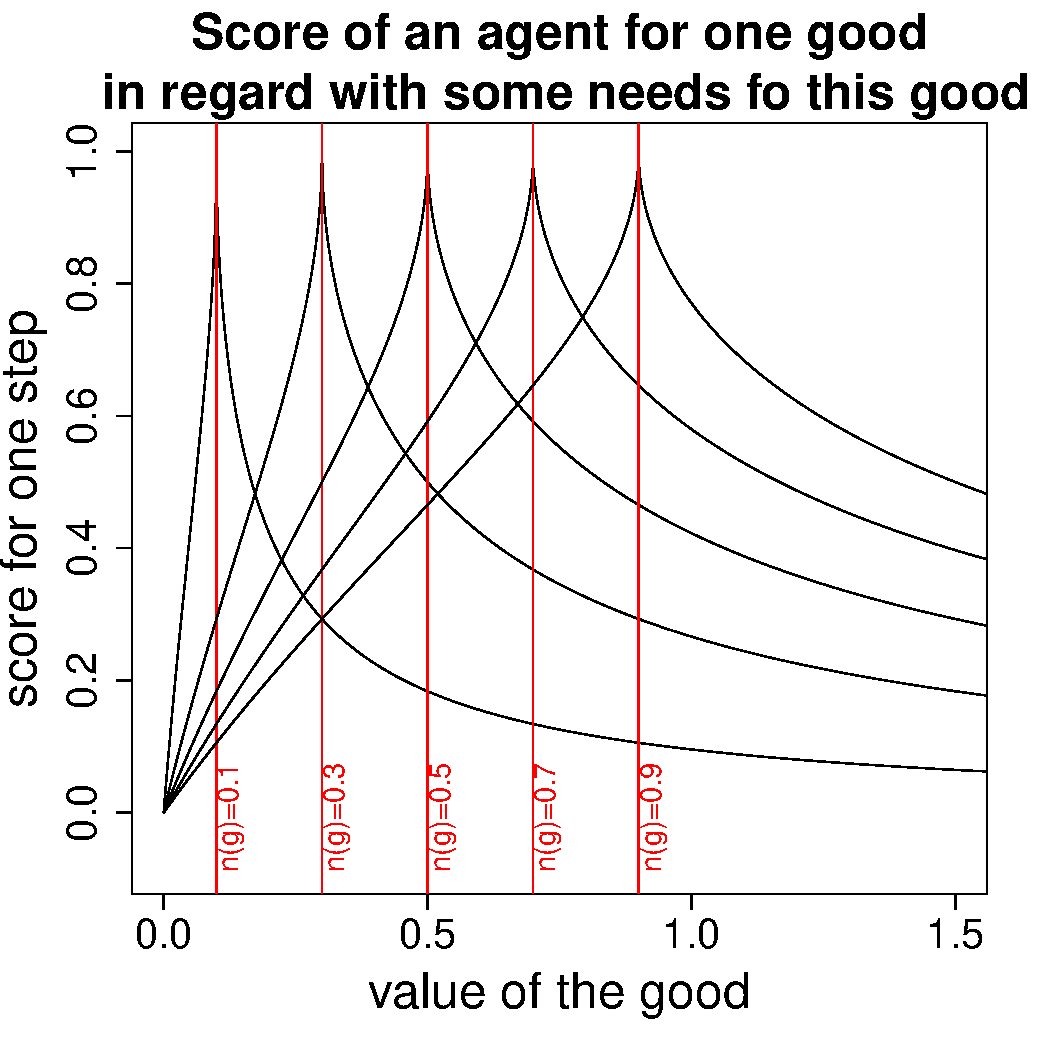
\includegraphics[width=7cm]{img/fitness.png}
	\end{center}
	\caption{The fitness depending on price and needs}
	\label{fig:fit}
\end{figure}

\todo{put a little description of what is in the figure}
The agents will choose the agent from whom the price vector should be copied among the agents that produce the same good and have the highest score. In practice, a fixed proportion of the less successful agents will copy the prices of the most successful agent. 

\paragraph{Trading} 


On top of producing goods, the agents have the ability to exchange them. During the trading phase the value associated to a good by an agent corresponds to the subjective price of the good for this agent. Briefly summarised, for each good that it does not produce, an agent will trade with the first parter that offer an acceptable trade, i.e. the agent that proposes a satisfiable ratio between the other product and the product produced by the agent. 

In more details, the trading phase starts by the agent looking at a first random agent producing another product. 
Let $o$ be an agent producing $g$ that proposes a trade and $r$ an agent producing $k$ that receives the proposition. As explained earlier, each has a quantity of good $Q^o$ and $Q^r$. On the one side, $o$ wants to exchange a quantity $w_g^o$ of the good $g$ for a quantity $w_k^o$ of the good $k$. On the other side, $r$ wants to exchange a quantity $w_g^r$ of the good $g$ for a quantity $w_k^r$. The tuples $W^o$ and $W^r$ describe the quantities of goods wanted by agent $o$ and $r$ for one trade proposition and are defined by:  

 $$ W^o=(w_g^o = v_g^o,w_k^o= \frac{v_k^o}{v_g^o}) $$ 
 $$ W^r=(w_k^r = v_k^r,w_g^r= \frac{v_g^r}{v_k^r}) $$

 Where $v_j^i$ are the estimated value of the good $j$ by the agent $i$ as defined earlier. 
The requested quantity of the non produced good is simply the ratio between the estimated value of the good requested and the estimated value of the produced good.


Once de quantities are defined, the agents declare that the trade is possible if :
\begin{align}
q_g^o >= w_g^o \\
q_g^r <= w_g^o \\
q_k^r >= w_k^o \\
w_g^o>=(q_g^r+w_g^r) \\
w_k^o<=w_k^r \\
w_g^o<=w_g^r
\end{align}


The conditions 2-4 insure that both agents have enough goods in their inventory to realise the trade and the conditions 5-7 insure that the quantities of each good fit the will of both agents.



If a trade is possible the two agents will exchange the agreed quantities. If the trade is not possible, the agent will continue to look at random partners for this good until either a good is found or $TradeThreshold$ agents have been tried. At this point the agent will try to trade with agents producing another good. The process goes on until all goods have been tried. This trading process is described in algorithm~\ref{algo:trade}.
%faire tableau parametre et y integrer Tradethreshold

\begin{algorithm}
\caption{Trading Process for agent $o$}
\label{algo:trade}
	\begin{algorithmic}[1]
	\scriptsize
		\For{$j \in Goods \And j \neq produced^i $}
			\State $tradeAttempt = 0$
			\For{$r \in Pop \And produced^r = j \And tradeAttempt < TradeThreshold $}
				\If{$acceptableTrade(W_o,W_r)$}
					\State $trade(W_o,W_r)$
				\Else
					\State $tradeAttempt = tradeAttempt + 1$					
				\EndIf
			\EndFor
		\EndFor
\end{algorithmic}
\end{algorithm}

%%deplacer et integrer dans 4.3
The trading process is performed at every iteration while the imitation and innovation processes are executed only every $CulturalStep$. The idea behind this is to perform the imitation based on a score that reflects the performance of the agent and not only one lucky or unlucky trading round.

\paragraph{Innovation} In a trading environment it seems unlikely that a price will change radically to a very different value. Therefore, a new and more realistic mechanism is proposed. The innovation process, termed ``self referenced'', is still triggered with a probability $\mu$ 
but modify the previous price by adding or subtracting a small amount taken randomly from a uniform  distribution between $0 .. \beta$.


\paragraph{Expected outcome} 

\todo{complete the equation}

With such a setup it is expected that the prices will converge to a ratio allowing each agent to obtain a number of resources equivalent to the needs. The best possible price of a good satisfies the equations :
\begin{align}
\frac{v^o_k}{v^o_g} = n_k \\
\frac{v^r_g}{v^r_k} = n_g \\
v^r_k = n_k \\
v^o_g = n_g \\
=>v^r_g = v^o_k = n_k * n_g \\
\end{align}

With as earlier, $o$ and $r$ the agents that respectively produces $g$ and $k$, $v_j^i$ the estimated value of the good $j$ for the agent $i$ and $n_j$ the needed value of the good $j$ for all agents.

If such prices are reached, all exchange can be done leading to a total score $S$ for each agent of the population : 
$$ S = \sum_{i=0}^{CulturalStep}  s^i(\tilde{Q}^i) \times ngoods $$ 
where $\tilde{Q}^i$ is the optimal quantity vector, i.e. the one for which $s^i(\tilde{Q}^i) = s_{max}$. Remember that from equation~\ref{eq:score}, $s_{max}=1$.


\subsection{Complete model}

The model used in these experiments, including the cultural transmission and trading mechanisms, is described in algorithms~\ref{algo:complete}

\begin{algorithm}
\caption{Model}
\label{algo:complete}
	\begin{algorithmic}[1]
	\scriptsize
	\State INITIALIZATION: 
		\For{$j \in Goods$}
			\For{$i \in \#Pop/\#Goods$} \Comment{Initialize the agent for the good it has to produce and a random value vector}
				\State $produced^i = j$
				\State $Q^i = (0, \cdots, 0)$
				\State $V^i = (v^i_0, \cdots, v^i_n)$ \Comment{The values of $v^i_j$ are selected randomly}
			\EndFor
		\EndFor

	\State SIMULATION:
		\Loop{$~step \in TimeSteps$}
			\For{$i \in Pop$}
				\State $Production()$
				\For{$j \in Pop$}
					\State $TradeProcess(i,j)$
				\EndFor				
				\If{$ (step \mod CulturalStep) = 0$}	
					\State $Imitation()$
					\State $Innovation()$
				\EndIf
			\EndFor
		\EndLoop
\end{algorithmic}
\end{algorithm}

\todo{upload and put an url, complete cite mare nostrum, put nb of hours per run (or the total)}
All experiments are performed with the simulator pandora~\cite{wittek_scalable_2012}. We have make the source code of our project available online~\footnote{put ulr}. All simulations presented are performed in the MareNostrumIII super computer~\cite{}, and took XXXh per run.

\jm{what about saying that we just count the iterations at the ``imitation, innovation step" ?}
In our experiment one has to take in account that agents modifies their prices or exchange their price only every $culturalStep$ steps. Between, twos such steps, the agent exchange goods given their own prices. Therefore we choose to run our simulation during 10000 step which correspond the 1000 time steps used by \cite{bentley_random_2004,mesoudi_random_2009}.

\todo{put the values in the table}

\begin{table}
\begin{center}
\begin{tabular}{@{}ll@{}}
\toprule
Parameter & Value \\
\midrule
Mutation probability & \\
Innovation probability & \\
CulturalStep &  10 \\
TradeThreshold & $\frac{Number of agent}{2}$ \\
TimeSteps & \\
\bottomrule
\end{tabular}
\caption{Table of parameters}\label{tab:parameters}
\end{center}
\end{table}


\section{RESULTS}
\subsection{Random cultural transmission and random innovation process}

We first analyse the result obtained in the ``neutral model" as presented in section~\ref{sec:}. The figure~\ref{fig:allMutation} presents an analysis of the value vectors obtained across the 100 runs performed with a $\mu$ value equal to XXXX. In this graph it is not the exact values that are analysed but their relative frequencies. The y-axis of the graph shows the frequencies of the variants of the vector values, the x-axis shows how many variant achieves such frequencies and the line represents the average of the frequencies obtained across all runs. Both axes are in a logarithmic scale

On this graphic one can observe a straight line which shows that a few of the variants are very frequent and a majority of them are not. Please note, that here the specific variant achieving high frequency is not studied, only the number of variants achieving such frequencies is presented. This line corresponds to the ``power law" distribution mentioned in section~\ref{sec:} and is typical of the result obtained under the ``neutral model". 

In order to further validate our model, we perform such study under various $\mu$ values as it has been done in previous works. The $\mu$ innovation rates studied vary $\in {.004,.008,.016,.064}$ and two population sizes are studied: 250 and 500 agents. The distribution of variants obtained is shown in figure~\ref{fig:allMutation}.

\begin{figure}[!hbp]
	\begin{center}
		\includegraphics[width=6cm]{img/allmuRandMaxN250.pdf}
		\includegraphics[width=6cm]{img/allmuRandMaxN500.pdf}
	\end{center}
	\caption{Distribution of frequencies depending on the $\mu$ parameter with 250 agents (left) and 500 agents (right)}
	\label{fig:allMutation }
\end{figure}

\jm{yes say the R package}
Under all parameters tested the value vectors exhibit power law like distribution. It would then be interesting to analyse the shape of such distribution. In order to perform this study a linear regression is used to fit the curve obtained to a function of the form $formul powerlaw$. The mean value of the $\alpha$ parameters obtained and their standard deviation is presented in table~\ref{tab:mualpha}. The computations of the linear regression is done thanks to PACKAGE

\begin{table}[h]
	\centering
	\begin{tabular}{ll|lllll}
		Agents Number & & Our result& & Bentley et al 2004\\
			&$\mu$ & $\alpha$ & SD&$\alpha$&SD\\\hline

		N = 250 
			&0.004&1.53&0.03&1.54&0.02\\
			&0.008&1.55&0.03&1.55&0.01\\
			&0.016&1.57&0.02&1.57&0.01\\
			&0.064&1.66&0.01&1.67&0.01\\\hline
		N= 500
		&0.004&1.50&0.02&1.53&0.03\\
		&0.008&1.52&0.02&1.57&0.01\\
		&0.016&1.55&0.03&1.61&0.04\\
		&0.064&1.78&0.08&1.81&0.10\\
	\end{tabular}
	\caption{Mean \& SD are calculate on 100 run.}
	\label{tab:mualpha}
\end{table}

\jm{Simon, do you have a comment on the table ? Like does it fit what is found in other articles ?}


\subsection{ Economical  process}

In order to study a trading model two new innovation and imitation mechanisms have been introduced as explained in section~\ref{sec:}. These mechanisms are summarized in the table~\ref{tab:exp}. Each couple of innovation/imitation mechanism form one setup that is labelled with one later. Note that the ``neutral model" studied in the previous section corresponds to the setup A. All the runs presented in this section are done for 100000 steps with a innovation rate $\mu=.004$ and $\beta=.001$.

\todo{add innovation and imitation}
\begin{table}[h]
	\centering
	\begin{tabular}{l|cc}
					&Imitation  Process \\
		Innovation Mechanism	& Rand & Success \\\hline  
		Unbounded 		&A & B \\
		Self Referenced	& C & D \\
	\end{tabular}
	\caption{Experimental Setup}
	\label{tab:exp}
\end{table}

\subsubsection{Distribution}


Our first step is to study the distribution of values in order to compare them to the distribution previous obtained. The distribution of values in the 4 setups is presented in figure~\ref{fig:4setDi}. 

\begin{figure}[H]
	\begin{center}
		\includegraphics[width=7cm]{img/frequenciesABCD.pdf}
	\end{center}
	\caption{Frequency distribution for the 4 setup}
	\label{fig:4setDi}
\end{figure}

\begin{table}[h]
	\centering
	\begin{tabular}{lcccc}
		& A & B & C & D\\
A & X& \includegraphics[width=5cm]{img/A-B.pdf}&\includegraphics[width=5cm]{img/A-C.pdf}&\includegraphics[width=5cm]{img/A-D.pdf}\\
B & X& X &\includegraphics[width=5cm]{img/B-C.pdf}&\includegraphics[width=5cm]{img/B-D.pdf}\\
C & X& X & X &\includegraphics[width=5cm]{img/C-D.pdf}\\
	\end{tabular}
	\caption{Experimental Setup}
	\label{tab:allRes}
\end{table}

\todo{update once all graphs are there}
\jm{is exponential law characteristic of prestige bias ?}

The results studied in the previous section is reproduce here in the by the setup A, it is therefore no surprise that this setup follow a power law. We observe that the setup D is also following a power law. However, setups B and C are following an exponential law. We therefore observe that the innovation process has a negligeable influence on the shape distribution. However, the use of a biased imitation process has a major effect on the shape of the distribution.



\subsubsection{Score}

We now study the setup in more detail by investigating the ability of the population of agents to find the good price to perform exchanges between each other. This is done by observing the score of all agents in each of the 4 setups. The results obtained are presented in figure~\ref{tab:scoreEvol}.

\begin{table}[H]
	\centering
	\begin{tabular}{l c c}
		& Random Transmission & Eco Transmission \\
		$\mu$ & \specialcell{\raisebox{-.5\height}{\includegraphics[width=5cm]{img/ScoreEvolutionForA-G2N250.pdf}}\\Setup A}&\specialcell{\raisebox{-.5\height}{\includegraphics[width=5cm]{img/ScoreEvolutionForB-G2N250.pdf}} \\ Setup B} \\
		$\mu + \alpha$& \specialcell{\raisebox{-.5\height}{\includegraphics[width=5cm]{img/ScoreEvolutionForC-G2N250.pdf}} \\ Setup C}&\specialcell{\raisebox{-.5\height}{\includegraphics[width=5cm]{img/ScoreEvolutionForD-G2N250.pdf}} \\ Setup D}

	\end{tabular}
	\caption{Evolution of the score in the different setup for typical run of each setup.}%%
	\label{tab:scoreEvol}
\end{table}

\todo{simon you have put A and S, I guess it's C and D ?}
\simon{It's A and C, the setup where their is no selection. But those two graph (A and B) are not good, don't take them in account. }
\todo{update explanation with new graphs}
\todo{get clear names for innovation and imitaiton mechanisms}
 
In the setups A and C, the score evolves randomly. In the two other setups however the score is increasing. Moreover, we observe that the XXXX innovation process used in the setups A and B leads to higher convergences. Since only the ``prestige imitation" takes the score into account it is normal that only this mechanism leads higher scores. The XXXX innovation mechanism leads to lower convergences as it select prices randomly in the complete range available.

\subsubsection{Prices}

We pursue the analysis of the economical aspect by observing the prices reached in setup D. As explained in the section~\ref{sec:} we expect that the trade imitation and innovation processes will produce a convergence toward a set of price for each good that will allow agents to exchange optimally the good they produce with the other goods. To verify this assumption we analyse the prices reached. These are presented in figure~\ref{fig:ratioEvol} as a deviation from the optimal price. Record that the optimal price is the ratio between the need of the needed good and the produced good.

\begin{figure}[H]
	\begin{center}
		\includegraphics[width=7cm]{img/ratioEvol.png}
	\end{center}
	\caption{Evolution of the difference $\dfrac{p(g_w)}{p(g_p)}-n(g_p)$ where $p(x_i)$ is the price for a good $i$, $n(x_i)$ its need, $g$ the produced good and $w$ the wanted}
	\label{fig:ratioEvol}
\end{figure}

We observe that prices are indeed converging to the optimal prices which means that our innovation and imitation process are valid trade mechanisms. Notably, they produce results similar to the ones obtained in~\cite{gintis_emergence_2006}.

\subsubsection{Suboptimal markets}

Finally, a more careful analysis of the price structure reveals the presence of suboptimal markets. In figure~\ref{fig:suboptimal} the price structure of one run of setup C is presented. The x-axis represents the number of iteration, the y-axis the prices. The green boxplot represents the price of good X for an agent producing Y. And the blue boxplot represents the price of good X for agent producince Y 

\begin{figure}[htp]
	\begin{center}
		\includegraphics[width=7cm]{img/suboptimal.png}
	\end{center}
	\caption{Evolution of the Score for the three types of agents of the simulation}
	\label{fig:suboptimal}
\end{figure}

In this graphic we can observe that the product displayed in green is blocked to a non-optimal value until iteration XXXX, and decreasing after. The prices for the blue product, on the other side, decrease steadily until the median reaches the uptimum at iteration XXXX. This illustrate the complexity of finding the right prices in the market. Indeed all prices are strongly linked together and until one has reach its optimum value, the other price can not evolve. 

\section{CONCLUSION}

This article has propose a framework to study both cultural transmission mechanisms and trade mechanisms. Our framework is based on a central element, the value vector, which is interpreted differently depending on the mechanisms studied. We have shown the validity of this approach by reproducing expected results on both the cultural and trade side. On the cultural transmission side we have shown that the implementation of the ``neutral model" leads to the expected observations on the variants of the vector value: a power law. When implementing trading mechanisms we observe the convergence of prices to the expected values and the improvement of the scores of the agents.

On top of these results, by the implementation of trade mechanisms as cultural mechanisms, we show that trade is plainly a cultural factor. The modifications needed in our framework where relative to the proposition of new imitation and innovation mechanisms which are typical of the study of the cultural transmission. This proximity between trade mechanisms and cultural transmission allows for the comparisons of the results obtained. For example, it has been possible here to compare the distribution of values obtained and highlight that the divergence from a power law actually is coming mainly from the imitation mechanism used in trade. Moreover this imitation mechanism can further be interpreted as a ``prestige bias" imitation already studied in cultural transmission.

\section{DISCUSSION}

%The questions we would like to ultimately study are for example: how does the hierarchical structure changes the adoption of a new product ? How delays and interruptions in the trade network change the culture of a society ?

In future works numerous, more realistic and complex dynamics can be studied in the same model. First the constraints on the production could be relaxed so that each agent can choose the products it wishes to produce at the current time step. Moreover, meterological factors can modify the quality of the production (noisy outcome of the process) thus making the process more realistic and more complex~\cite{bentley_specialisation_2005}.

The goods themselves can be of different type: ``vital'' or ``common''. The absence of a ``vital'' good would then lead to the death of the agent. Thus making the need to trade at the best price even stronger for the agent. The ``common'' goods on the other sides would be interesting to observe the evolution of a culture out of the necessity of survival. The mechanisms behind the strong use of a non-essential product can then be studied. Naturally in the study of these questions the consumption function would change trough time for the agent.

The trading theories studied also can be extended to the \emph{Prospect Theory}~\cite{kahneman_prospect_1979} which proposes to study more realistic trade mechanisms taking into account the biases of humans. Another economical framework we envision is the Agent based Computational Economy, ACE, which is  addressing economical problems raising from the interactions of a large number of agents~\cite{tesfatsion_introduction_2001}. On top of these trading theories the influence of the network of trades by itself can be studied. Various networks can be envisioned ranging from fully connected to small world, and taking into account possible delays or the sudden rupture of a link.


On the cultural transmission side, the vector value could be learned using any mechanism of ``social learning'' (as defined by \cite{lycett_cultural_2015}) known in the literature (teaching, different kind of copying mechanisms,\ldots) and/or integrate any cognitive/environmental bias that could be studied (see again \cite{lycett_cultural_2015} for some kind of bias that could be implemented). Agents could be also endowed with self-adaptation abilities implemented thanks to Reinforcement Learning or Developmental Learning. Another possible track to implement the self-adaptation abilities is to rely on the cognitive approaches that propose to model the complexity of the human behaviour in general representations such as BDI.


\bibliographystyle{wsc}
\bibliography{wsc.bib}  
\end{document}

